\begin{enumerate}

  \item \textbf{ELEMENTO\_GEOLÓGICO} (supertipo): \texttt{id\_elemento\_geológico} (llave).
	\item \textbf{RÍO} (subtipo de \textit{ELEMENTO\_GEOLÓGICO}): \texttt{nombre}, \texttt{descripción}, \texttt{longitud\_total}.
	\item \textbf{MONTAÑA} (subtipo de \textit{ELEMENTO\_GEOLÓGICO}): \texttt{nombre}, \texttt{descripción}, \texttt{altura}.
	\item \textbf{MONTAÑA\_VOLCÁNICA} (subtipo de \textit{MONTAÑA}): \texttt{tipo\_volcán}.
	\item \textbf{MONTAÑA\_PLEGAMIENTO} (subtipo de \textit{MONTAÑA}): \texttt{periodo\_geológico}.
	\item \textbf{MUNICIPIO}: \texttt{id\_municipio} (llave), \texttt{nombre}, \texttt{num\_habitantes}.
	\item \textbf{SISTEMA\_MONTAÑOSO}: \texttt{código} (llave), \texttt{nombre}, \texttt{orientación} \{norte, sur, este, oeste\}, \texttt{longitud}, \texttt{altura\_máxima}.
	\item \textbf{SATÉLITE}: \texttt{id\_satélite} (llave), \texttt{nombre}, \texttt{descripción}.
	\item \textbf{ATRAVIESA} (relación N:M entre \textit{RÍO} y \textit{MUNICIPIO}, atributo \texttt{longitud\_tramo}): participación total de \textit{RÍO}, parcial de \textit{MUNICIPIO}.
	\item \textbf{ES\_AFLUENTE\_DE} (relación ternaria recursiva entre \textit{RÍO}, \textit{RÍO} y \textit{MUNICIPIO}): roles \texttt{afluente} (0,1), \texttt{recibe} (0,N) y \texttt{confluencia} (0,N).
	\item \textbf{PERTENECE\_A} (relación N:1 entre \textit{MONTAÑA} y \textit{SISTEMA\_MONTAÑOSO}): participación total de \textit{MONTAÑA}; \textit{SISTEMA\_MONTAÑOSO} es el lado de cardinalidad 1.
	\item \textbf{OCUPA} (relación N:M entre \textit{SISTEMA\_MONTAÑOSO} y \textit{MUNICIPIO}): participación total de \textit{SISTEMA\_MONTAÑOSO}, parcial de \textit{MUNICIPIO}.
	\item \textbf{SE\_ENCUENTRA\_EN} (relación N:M entre \textit{MONTAÑA} y \textit{MUNICIPIO}): participación total de \textit{MONTAÑA}, parcial de \textit{MUNICIPIO}.
	\item \textbf{MONITOREA} (relación 1:N entre \textit{SATÉLITE} y \textit{ELEMENTO\_GEOLÓGICO}, atributo \texttt{fecha\_inicio\_monitoreo}): \textit{SATÉLITE} es el lado de cardinalidad 1; participación parcial de \textit{ELEMENTO\_GEOLÓGICO}.

  
\end{enumerate}

% ==========================================
% Modelo E-R (página en horizontal, tamaño carta)
% ==========================================
\clearpage
% Página tamaño carta en horizontal: se fija el tamaño físico de la página y se
% centra el diagrama, dejando 1 cm de margen por lado.
\pdfpagewidth=11in
\pdfpageheight=8.5in
\setlength{\textwidth}{\dimexpr\pdfpagewidth-2cm\relax}
\setlength{\hsize}{\dimexpr\pdfpagewidth-2cm\relax}
\setlength{\oddsidemargin}{\dimexpr(\pdfpagewidth-\textwidth)/2 - 1in\relax}
\setlength{\evensidemargin}{\oddsidemargin}
\setlength{\textheight}{\dimexpr\pdfpageheight-2cm\relax}
\setlength{\vsize}{\dimexpr\pdfpageheight-2cm\relax}
\setlength{\headheight}{0pt}
\setlength{\headsep}{0pt}
\setlength{\topmargin}{\dimexpr(\pdfpageheight-\textheight)/2 - 1in\relax}
\thispagestyle{empty}
\vspace*{\fill}
\centering
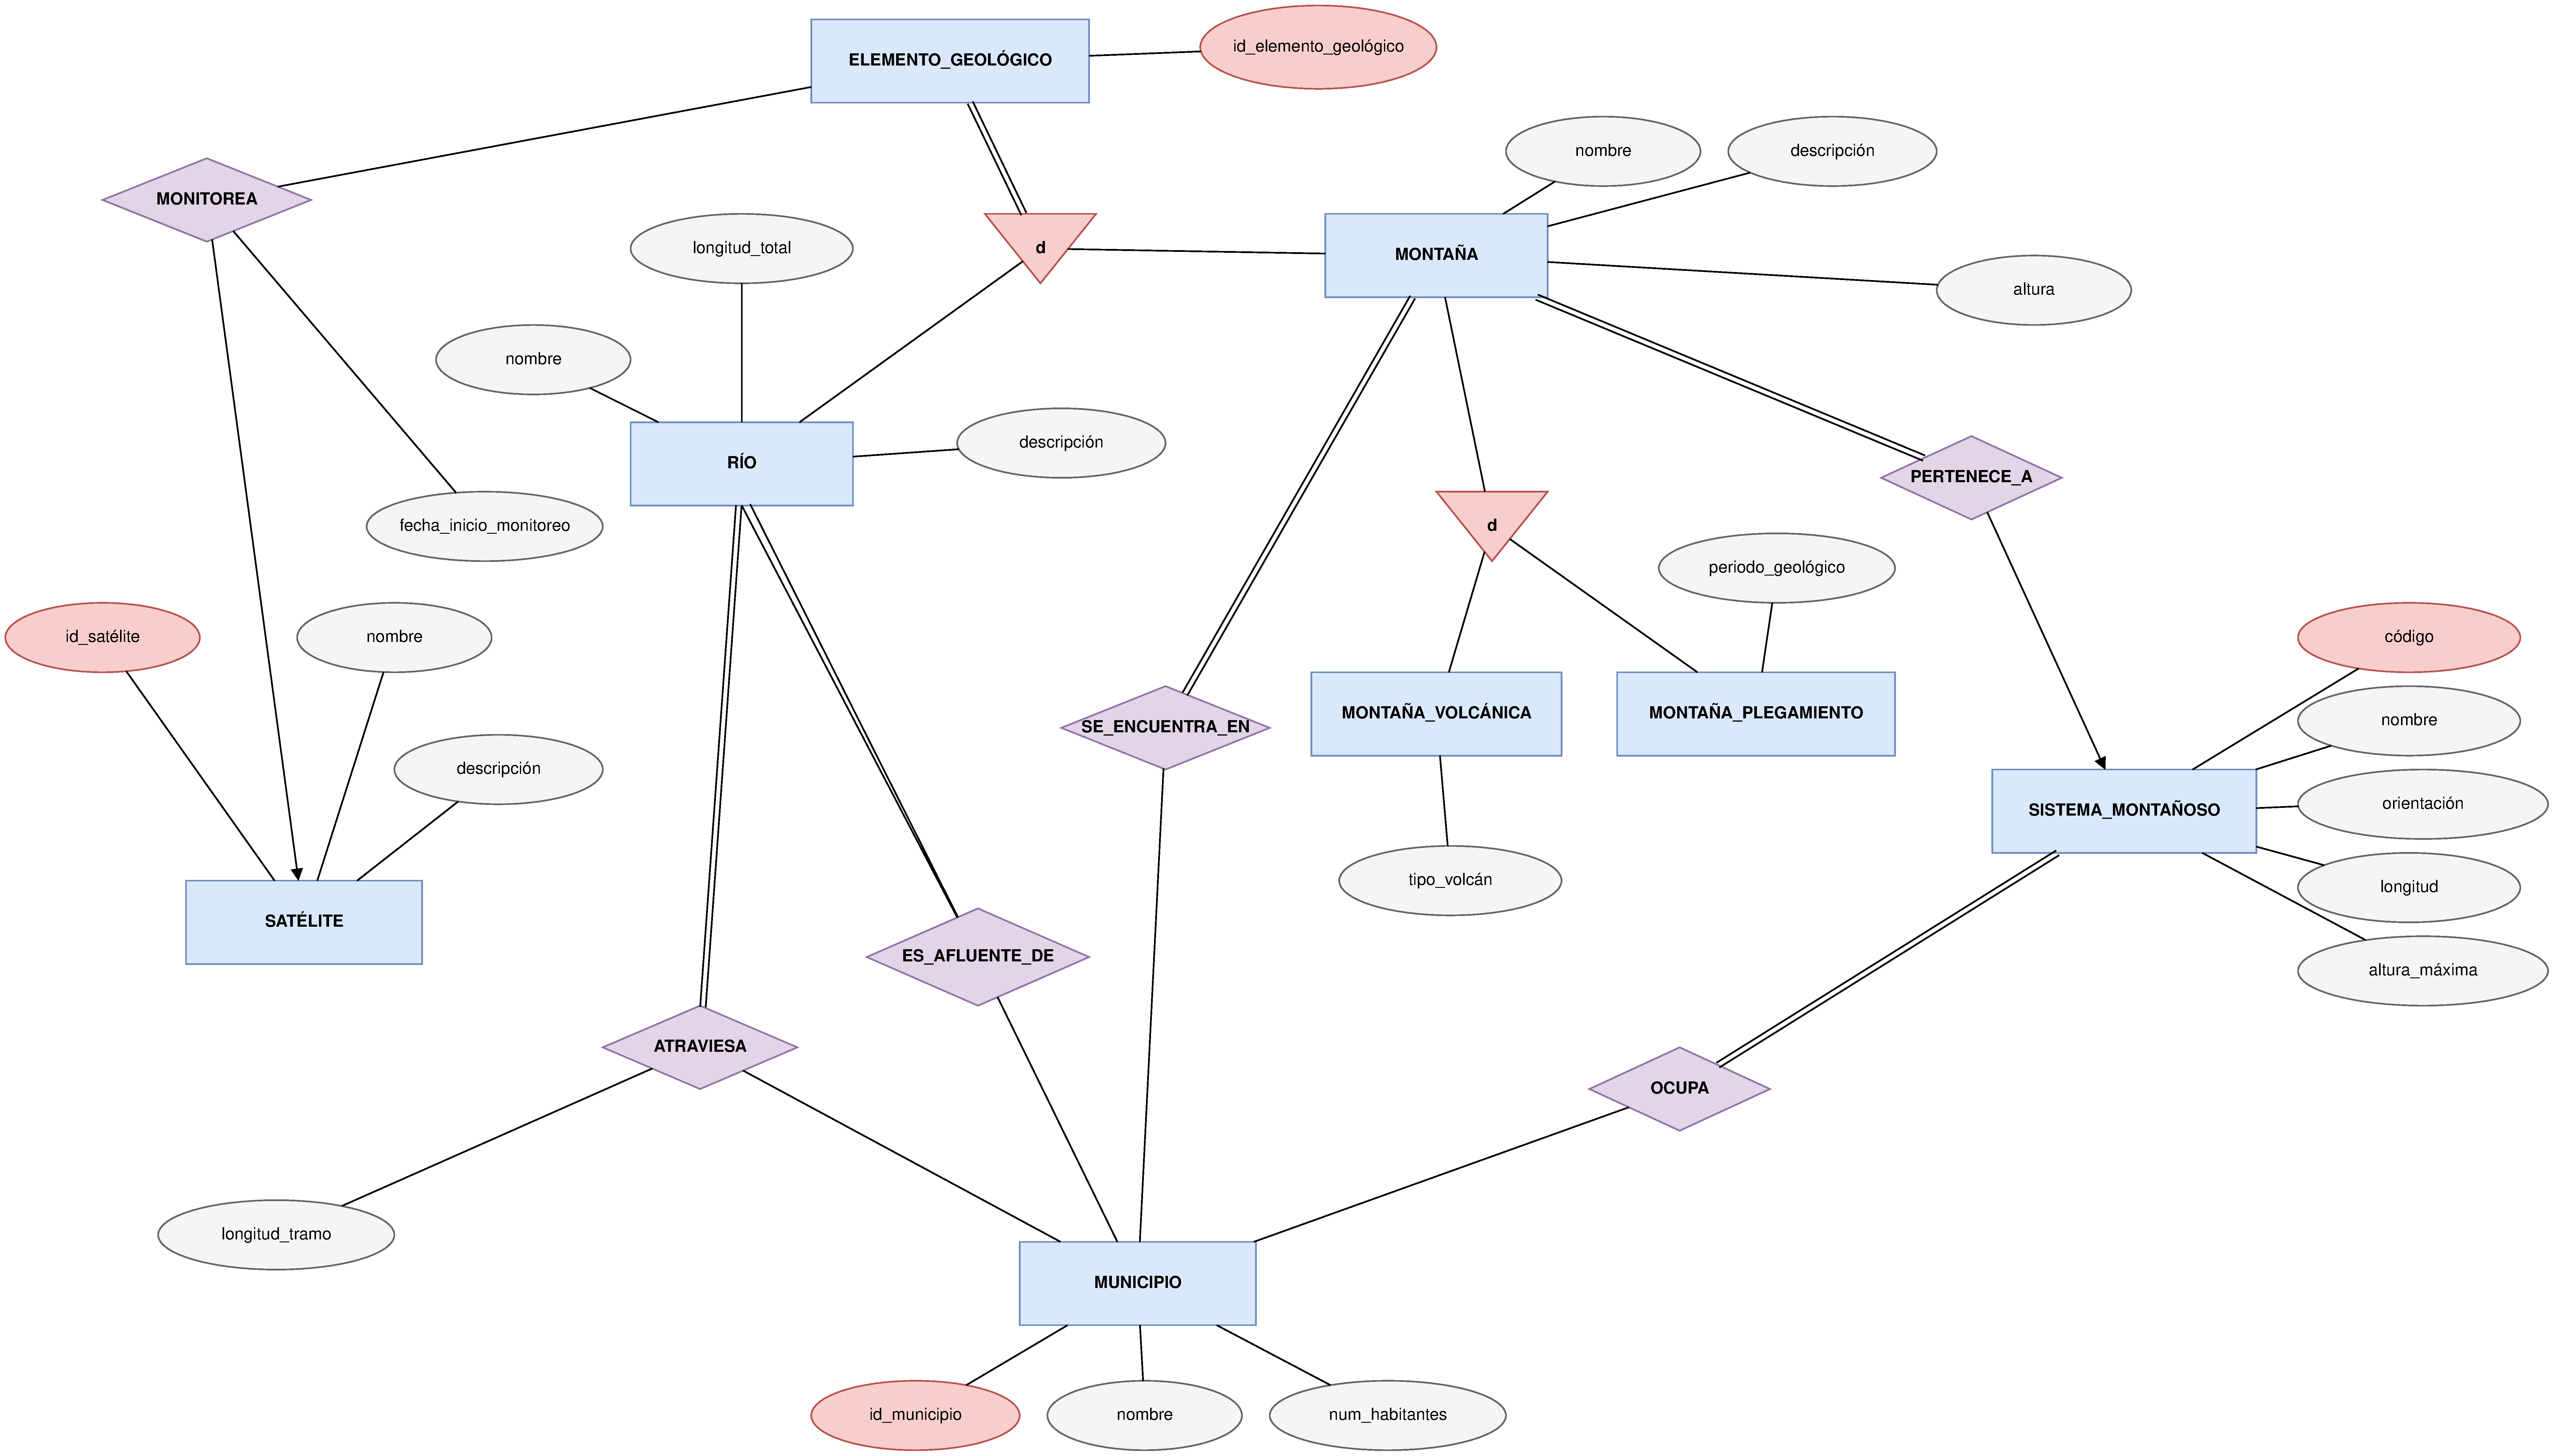
\includegraphics[width=\textwidth, height=0.85\textheight, keepaspectratio]{Figuras/3c.pdf}
\captionof{figure}{Modelo E-R para Sistema de Informacion Geografica.}
\label{fig:er_3c}
\vspace*{\fill}
\clearpage
\restoregeometry
\pdfpagewidth=\paperwidth
\pdfpageheight=\paperheight

\subsection*{Consideraciones para Modelo Relacional}

\begin{enumerate}

\item \textbf{Satélite}: Su llave primaria es \textit{id\_satélite}, perteneciente al dominio de los enteros (\textit{int}) y cuenta con una restricción de integridad de entidad (\textbf{NOT NULL}, \textbf{UNIQUE}). Sus atributos \textit{nombre} y \textit{descripción} operan bajo el dominio de cadena de caracteres (\textit{varchar}) con restricción de integridad de dominio (\textbf{NOT NULL}).

\item \textbf{Municipio}: Su llave primaria es \textit{id\_municipio}, con dominio \textit{int} y restricción de integridad de entidad (\textbf{NOT NULL}, \textbf{UNIQUE}). Los atributos \textit{nombre} (\textit{varchar}) y \textit{num\_habitantes} (\textit{int}) operan con restricción \textbf{NOT NULL}.

\item \textbf{Sistema\_Montañoso}: Su llave primaria es \textit{código}, asumiendo un dominio \textit{varchar} o \textit{int}, con restricción estricta de integridad (\textbf{NOT NULL}, \textbf{UNIQUE}). Sus atributos \textit{nombre} y \textit{orientación} pertenecen al dominio \textit{varchar}, mientras que \textit{longitud} y \textit{altura\_máxima} adoptan el dominio \textit{decimal} (o \textit{int}), todos contando con restricciones de integridad de dominio (\textbf{NOT NULL}).

\item \textbf{Elemento\_Geológico} (Supertipo): Esta tabla funge como el supertipo creado para simplificar los identificadores de \textbf{Río} y \textbf{Montaña}, y para evitar duplicar la relación MONITOREA. Su llave primaria es \textit{id\_elemento\_geológico}, perteneciente al dominio de los enteros (\textit{int}) con restricción (\textbf{NOT NULL}, \textbf{UNIQUE}).
Al tener una cardinalidad 1:N en su asociación MONITOREA con \textbf{Satélite}, la tabla absorbe la llave de dicha entidad. Por lo tanto, integra la llave foránea (FK) \textit{id\_satélite} (\textit{int}) aplicando integridad referencial hacia \textbf{Satélite}. Dado que la participación de \textbf{Elemento\_Geológico} en esta relación es parcial, esta llave foránea admite valores nulos (\textbf{NULL}). Finalmente, el atributo de la relación, \textit{fecha\_inicio\_monitoreo}, es arrastrado hacia esta tabla operando bajo el dominio \textit{date}.

\item \textbf{Especialización total disjunta} (Río y Montaña): El modelo E-R presenta una jerarquía de generalización/especialización total disjunta para la superentidad \textbf{Elemento\_Geológico} en las subentidades \textbf{Río} y \textbf{Montaña}. Se crea una tabla para cada una de las dos subentidades. Ambas incorporan como llave primaria el atributo \textit{id\_elemento\_geológico} (\textit{int}), que actúa simultáneamente como llave foránea (FK) hacia la superentidad \textbf{Elemento\_Geológico} con estricta integridad referencial.
\begin{itemize}
    \item \textbf{Río}: Recibe los atributos propios \textit{nombre}, \textit{descripción} (\textit{varchar}) y \textit{longitud\_total} (\textit{decimal}) con restricción \textbf{NOT NULL}.
    \item \textbf{Montaña}: Recibe los atributos \textit{nombre}, \textit{descripción} (\textit{varchar}) y \textit{altura} (\textit{decimal}). Adicionalmente, al participar en la relación N:1 (PERTENECE\_A) con participación total hacia \textbf{Sistema\_Montañoso}, esta tabla absorbe la llave de dicha entidad. Por tanto, integra la llave foránea (FK) \textit{código} (\textit{varchar}) con restricción de integridad referencial y restricción \textbf{NOT NULL}.
\end{itemize}

\item \textbf{Especialización disjunta} (Montaña\_Volcánica y Montaña\_Plegamiento): Existe una segunda jerarquía de especialización disjunta a partir de \textbf{Montaña}. Las tablas resultantes, \textbf{Montaña\_Volcánica} y \textbf{Montaña\_Plegamiento}, heredan como llave primaria y foránea (FK) simultánea a \textit{id\_elemento\_geológico} (\textit{int}), asegurando la integridad referencial hacia \textbf{Montaña}.
\begin{itemize}
    \item \textbf{Montaña\_Volcánica}: Aloja el atributo \textit{tipo\_volcán} (\textit{varchar}) con restricción \textbf{NOT NULL}.
    \item \textbf{Montaña\_Plegamiento}: Aloja el atributo \textit{periodo\_geológico} (\textit{varchar}) con restricción \textbf{NOT NULL}.
\end{itemize}

\item \textbf{Atraviesa}: Esta tabla surge de la conversión de una cardinalidad de muchos a muchos (N:M) entre \textbf{Río} y \textbf{Municipio}. Su llave primaria es compuesta por los identificadores de las entidades que conecta: \textit{id\_elemento\_geológico} (FK hacia \textbf{Río}) e \textit{id\_municipio} (FK hacia \textbf{Municipio}). Ambas imponen restricciones de integridad referencial. Se incorpora a esta tabla el atributo de la relación \textit{longitud\_tramo}, bajo el dominio \textit{decimal} con restricción \textbf{NOT NULL}.

\item \textbf{Ocupa}: Al ser una relación muchos a muchos (N:M) entre \textbf{Sistema\_Montañoso} y \textbf{Municipio}, se crea esta tabla de intersección. Su llave primaria es compuesta por \textit{código} (FK hacia \textbf{Sistema\_Montañoso}) e \textit{id\_municipio} (FK hacia \textbf{Municipio}), ambas manteniendo integridad referencial estricta.

\item \textbf{Se\_Encuentra\_En}: Al igual que las anteriores, surge de la cardinalidad muchos a muchos (N:M) entre \textbf{Montaña} y \textbf{Municipio}. Su llave primaria es compuesta por \textit{id\_elemento\_geológico} (FK hacia \textbf{Montaña}) e \textit{id\_municipio} (FK hacia \textbf{Municipio}), aplicando restricciones de integridad referencial.

\item \textbf{Es\_Afluente\_De}: Se crea a partir de una relación ternaria recursiva con cardinalidad M:N entre las entidades \textbf{Río} (que participa con dos roles) y \textbf{Municipio}. Su llave primaria es compuesta por los identificadores de los tres roles involucrados: \textit{id\_afluente} (FK hacia \textbf{Río}, dominio \textit{int}), \textit{id\_recibe} (FK hacia \textbf{Río}, dominio \textit{int}) e \textit{id\_municipio} (FK hacia \textbf{Municipio}, dominio \textit{int}). Las tres columnas aplican restricciones estrictas de integridad referencial hacia sus respectivas tablas de origen.

\end{enumerate}

% ==========================================
% Modelo Relacional (página en horizontal, tamaño carta)
% ==========================================
\clearpage
\pdfpagewidth=11in
\pdfpageheight=8.5in
\setlength{\textwidth}{\dimexpr\pdfpagewidth-2cm\relax}
\setlength{\hsize}{\dimexpr\pdfpagewidth-2cm\relax}
\setlength{\oddsidemargin}{\dimexpr(\pdfpagewidth-\textwidth)/2 - 1in\relax}
\setlength{\evensidemargin}{\oddsidemargin}
\setlength{\textheight}{\dimexpr\pdfpageheight-2cm\relax}
\setlength{\vsize}{\dimexpr\pdfpageheight-2cm\relax}
\setlength{\headheight}{0pt}
\setlength{\headsep}{0pt}
\setlength{\topmargin}{\dimexpr(\pdfpageheight-\textheight)/2 - 1in\relax}
\thispagestyle{empty}
\vspace*{\fill}
\centering
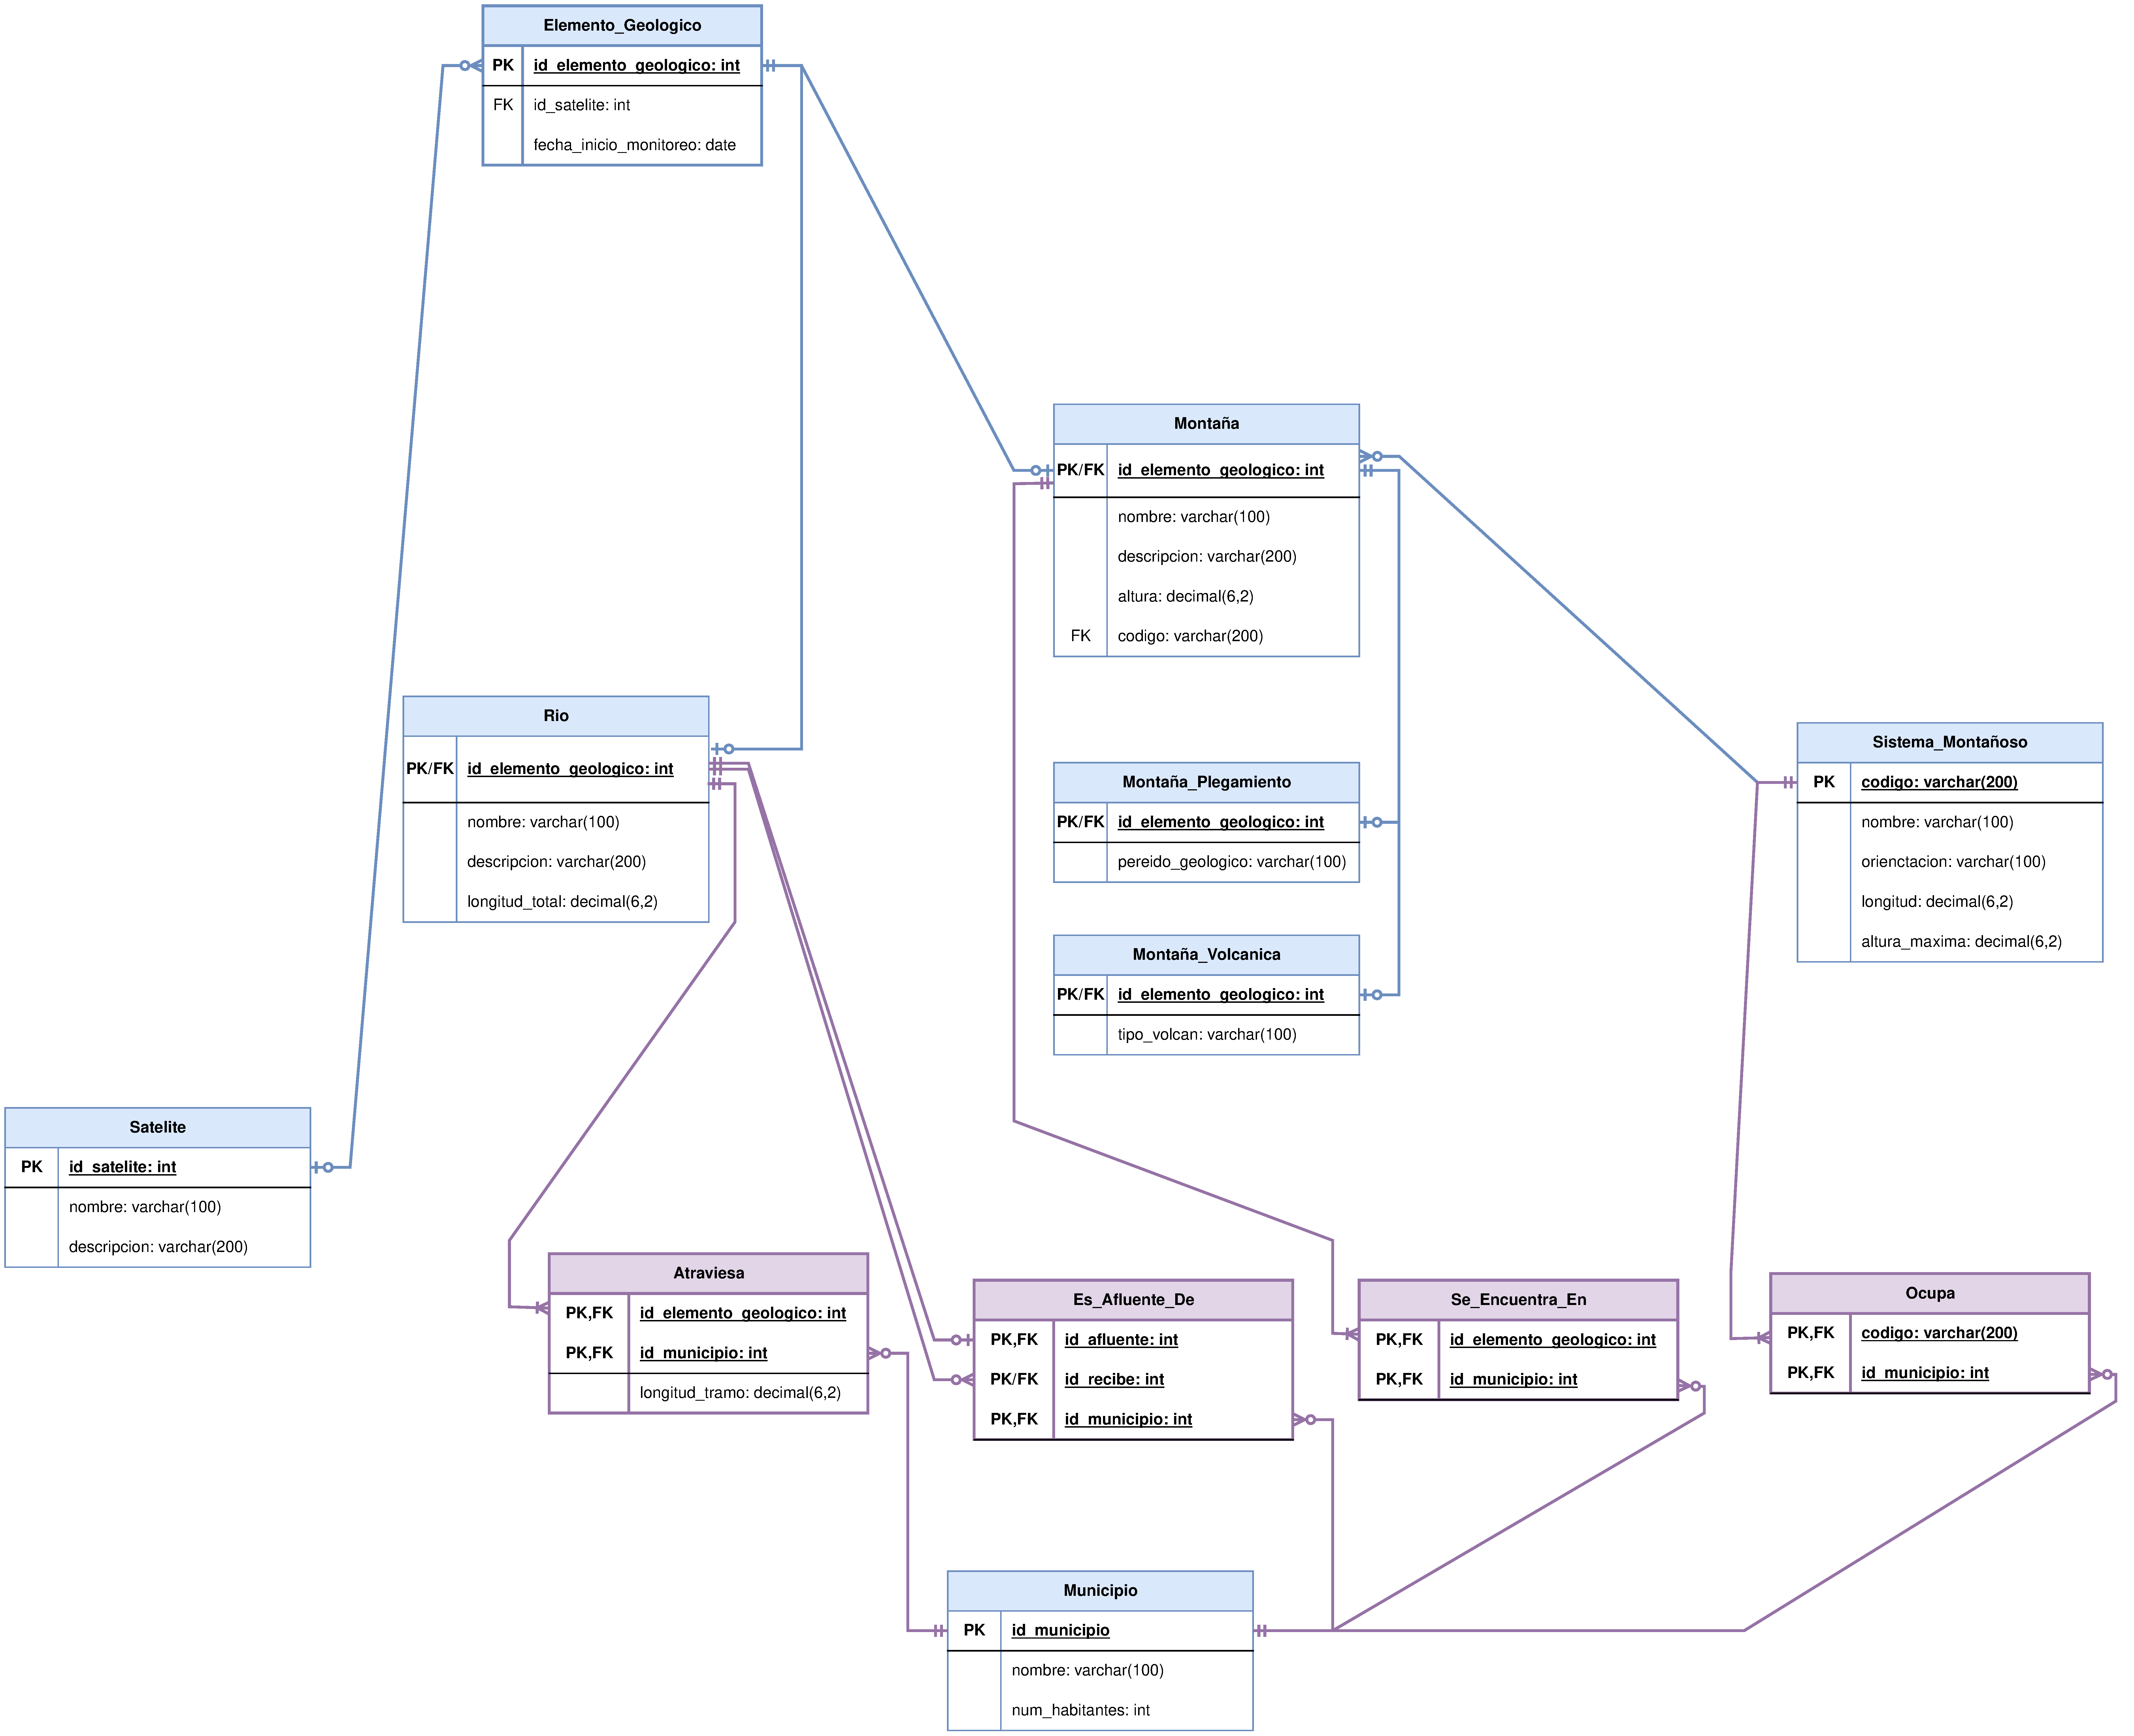
\includegraphics[width=\textwidth, height=0.85\textheight, keepaspectratio]{Figuras/RelacionalT2E3c.pdf}
\captionof{figure}{Modelo Racional para Sistema de Informacion Geografica.}
\label{fig:rel_3c}
\vspace*{\fill}
\clearpage
\restoregeometry
\pdfpagewidth=\paperwidth
\pdfpageheight=\paperheight
